\chapter{The Waveform as the Observation}\label{ch:phase3}\label{app:phase3}\label{sec:phase3-math}
The waveform setting is stage 3 of the thesis's progression: the
observation becomes the waveform itself, the endpoint toward which the
piano and strings-and-winds settings were built. Every study in this chapter is exploratory and was conducted on
the development set, and no evaluation of the waveform setting on a held-out
test set has been performed (the protocol is described in
\S\ref{sec:hygiene}). The chapter nevertheless belongs to the main line of
the thesis, because the waveform setting is the most novel step of the
programme and because its design constraints have now been quantified on
real audio rather than assumed.

The audio likelihood replaces the per-note observation $\tilde y$ with the
waveform $x \in \R^{M}$:
\begin{equation}
  x \;=\; \Phi(z)\, a + \epsilon, \qquad \epsilon \sim \N(0,\, K_n),
  \label{eq:waveform}
\end{equation}
where $z$ collects the nonlinear position variables (tempo, timing,
intonation, vibrato), $\Phi(z) \in \R^{M \times 2HN}$ is the deterministic
harmonic synthesis basis, and $a \in \R^{2HN}$ are the stacked per-note
harmonic amplitudes. The basis is the horizontal concatenation of one
$M \times 2K$ block per note, with quadrature columns
$\cos\phi_k(t), \sin\phi_k(t)$ and cumulative phase
$\phi_k(t) = 2\pi k \int_0^t f_0(s)\, ds$ determined by $z$, where $H$ counts
the harmonics. Per-note amplitudes are shaped in time by an amplitude
envelope $A_i(t)$, which multiplies the columns of $\Phi(z)$ belonging to
note $i$. One asymmetry of this specification should be stated at the
outset. Loudness lives in the amplitudes $a$ and articulation in the
envelope supports, and neither is placed under the graph prior. Assigning
every per-note channel of the previous chapters a home, in $z$, in $a$ or
in $A_i$, with its structure stated, is part of designing the waveform
setting in full rather than a detail. With a Gaussian amplitude prior
$a \sim \N(\mu_a, \Sigma_a)$, the amplitudes marginalise exactly:
\begin{align}
  p(a \mid x, z) &= \N(m_a,\, S_a), \qquad
  S_a = \bigl( \Sigma_a^{-1} + \Phi^\top K_n^{-1} \Phi \bigr)^{-1}, \qquad
  m_a = S_a \bigl( \Sigma_a^{-1} \mu_a + \Phi^\top K_n^{-1} x \bigr),
  \label{eq:amp-post}\\[2pt]
  p(x \mid z) &= \N\bigl( x;\; \Phi\, \mu_a,\; \Phi\, \Sigma_a\, \Phi^\top + K_n \bigr),
  \label{eq:collapsed}
\end{align}
where $\Phi = \Phi(z)$, $\mu_a \in \R^{2HN}$ and
$\Sigma_a \in \R^{2HN \times 2HN}$ for $H$ harmonics with two quadrature
columns each. The implementation specialises the noise covariance to
$K_n = \sigma^2 I$, and the amplitude envelope $A_i(t)$ belongs to the
specification but is not yet implemented. Inference over the nonlinear $z$,
by a Laplace approximation or by variational inference initialised from the
nominal score, is the open step. The coupled graph prior, the first two
terms of \eqref{eq:gpfirst}, plays the role of the structured component of
$p(z)$.

\figph{arch_phase3.pdf}{1.0}{The waveform system. Dashed: the joint
whole-performance system is not yet implemented. The likelihood block is
exercised in \S\ref{sec:phase3-study}, and the prior's first span inside it
in \S\ref{sec:phase3-priorvalue}. The observation is the waveform itself.
The same joint kernel now serves as the prior over $z$, the likelihood block
becomes the marginalised audio likelihood
$p(x \mid z) = \N\bigl(\Phi\mu_a,\ \Phi\Sigma_a\Phi^{\top} + K_n\bigr)$, and
the head is the one non-conjugate element (Laplace or variational inference
over $z$, with the amplitudes recovered in closed form). Relative to
Figure~\ref{fig:arch-phase1} the likelihood has moved and the inference head
has become approximate, while the prior branches carry
over.\label{fig:arch-phase3}}

\section{Scalar intonation from the waveform}
\label{sec:phase3-study}

The collapsed likelihood \eqref{eq:collapsed} was first applied to real
audio in a development study designed to answer two questions. The first is
whether the waveform carries the per-note expressive information directly,
with no pitch tracker in the loop. The second is whether the resulting
posterior is calibrated. The study is exploratory, its evidence is confined
to the development set, and its outcome, a gap between the quantity the
waveform model estimates and the quantity the reference defines, shapes the
design of everything that follows in this chapter.

\subsection{Design of the single-note study}

One observation is one note's audio segment of $m$ samples at $16$\,kHz, up
to two seconds long ($m \approx 10^{3.5}$--$10^{4.5}$), cut at the annotated
note boundaries of a development URMP track. The study covers $376$ notes
from seven tracks spanning all three instrument families. For each note the
$f_0$ curve is parameterised by the variables of the six-channel bundle
(eqs.~\eqref{eq:cents-curve}--\eqref{eq:vibrato}). On vibrato-identifiable
notes the extent, rate and delay scaffold is taken from the per-note
estimator of Chapter~\ref{ch:phase2}, the one estimator-supplied ingredient
of the study. The design matrix is the harmonic basis of \eqref{eq:waveform}
with amplitudes piecewise constant over the four chunks of
\eqref{eq:loudness}, giving $p = 2H \times 4 = 64$ columns at $H=8$
harmonics. The amplitudes are marginalised exactly, and an $O(mp^{2})$
Woodbury form of \eqref{eq:collapsed}, whose equality with the dense form is
verified in unit tests, keeps the segment-length likelihoods tractable.

Inference over the intonation centre $c$ is by grid search, with a coarse
pass at $1$-cent spacing over $\pm 50$ cents around the score-nominal pitch
followed by a fine refinement at $0.03$ cents ($0.06$ for the deviation
variant). This is exact 1-D inference up to discretisation, and no Laplace
approximation is involved. Four position models are compared. The first is a
constant $c$. The second adds AR(1) observation noise, a residual whitening
with the correlation fitted per note. The third adds the linear drift term
of the \S\ref{sec:phase2} drift study, with the slope profiled on a grid.
The fourth adds a marginalised pitch-curve deviation prior of eight
zero-mean Hann bumps along the curve Jacobian, with a prior standard
deviation of $5$ cents per coefficient, treated exactly like the amplitudes.
Each posterior is scored against the reference centre, the per-note NLLS
estimator applied to the corpus's annotated pitch curve, by absolute error
and by coverage at nominal $90\%$. A fifth condition calibrates the
machinery itself on synthetic notes built from real notes' fitted structure,
for which the model is true by construction.

\begin{table}[t]\centering
\caption{Inference of the intonation centre from the waveform on $376$ real
notes from seven development tracks across three instrument families, with
no pitch tracker in the loop. The score is the distance to the reference
centre, and coverage is at nominal $90\%$. The estimator row is the full
pyin-plus-NLLS chain of Chapter~\ref{ch:phase2}, and the last row is the
self-check on model-true synthetic notes. All rows are exploratory results
on the development set.}
\label{tab:phase3-study}
\footnotesize
\begin{tabular}{@{}lccc@{}}
\toprule
position model & median $|$err$|$ (cents) & q90 & coverage@90 \\
\midrule
constant $c$ & 2.81 & 8.72 & 0.03 \\
$+$ AR(1) noise & 2.73 & 8.37 & 0.02 \\
$+$ drift term & 2.40 & 7.23 & 0.01 \\
$+$ deviation prior & 2.29 & 6.77 & 0.03 \\
\midrule
pyin $+$ NLLS estimator chain & 2.01 & --- & (supplies its own $\sigma$) \\
model-true synthetics (self-check) & --- & --- & \textbf{0.90} \\
\bottomrule
\end{tabular}
\end{table}

\begin{figure}[t]
  \centering
  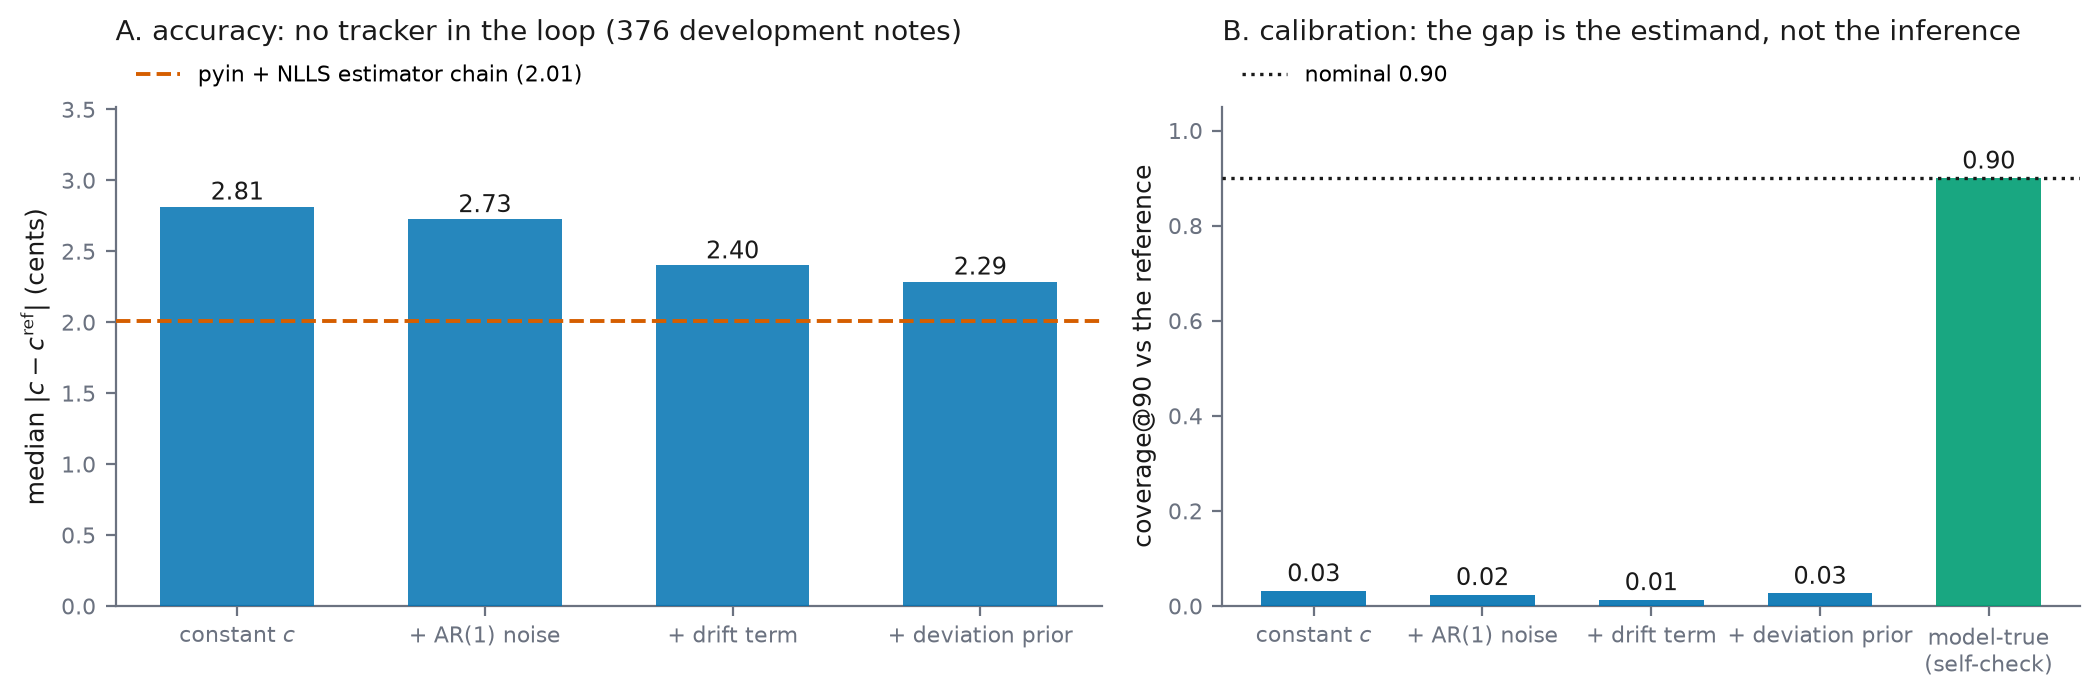
\includegraphics[width=\linewidth]{figures/phase3_study_dev.png}
  \caption{The waveform study on the development set. Panel A: the median
  distance to the reference intonation centre for each position-model
  refinement, with the dedicated estimator chain dashed and the wind family
  shown separately ($2.67$ vs $3.27$ cents). Panel B: coverage against the
  reference for every variant, together with the coverage of the same
  machinery on model-true synthetic notes (green).}
  \label{fig:phase3-study}
\end{figure}

\subsection{Accuracy and calibration against the reference}

Three facts are visible in Table~\ref{tab:phase3-study} and
Figure~\ref{fig:phase3-study}. First, the waveform carries the information.
The best variant reaches a median of $2.29$ cents from the reference,
approaching the estimator chain's $2.01$ overall and improving on it on the
winds ($2.67$ vs $3.27$), the family in which the tracker's failure modes
are concentrated. The two-note pilot that preceded the study showed the same
at $0.7$--$1.6$ cents on long clean notes. Second, every model refinement
improves accuracy, yet coverage against the reference is invariant at
$0.01$--$0.03$. The drift term of the \S\ref{sec:phase2} study transfers to
the waveform domain (paired median $-0.18$ cents), and the deviation prior
improves accuracy further. A better mean model, however, shrinks the
posterior width as fast as it shrinks the error, and the AR(1) floor does
not help, because the structured misfit is concentrated \emph{in band}, at
the harmonics, where a stationary coloured floor cannot reach. Third, the
machinery itself is calibrated: on model-true synthetic notes the same
posterior covers at exactly $0.90$ (median $|z| = 0.53$).

\subsection{The estimand gap and its consequence for the bundle}

Together these three facts locate the overconfidence. It is an
\textbf{estimand gap}: the constant the harmonic model estimates and the
constant the NLLS estimator defines on the annotated curve are different
functionals of the same performance, about two cents apart, and no
within-model refinement can close a gap between two different questions,
which is why none of the three refinements did. The design conclusion
follows. The waveform posterior should enter the six-channel bundle the way
every estimator does, as a measurement whose noise row is its posterior
variance plus an empirically calibrated per-note discrepancy floor at the
observed $\sim 2$-cent scale. This restores calibration by construction
under the convention, used throughout the bundle, that each estimator's own
variances are taken as its noise row.

A first integration study on the same seven tracks, also exploratory,
implements exactly this design. The waveform posterior enters as a seventh
bundle channel, its coupling is learned per piece by the evidence, and the
discrepancy floor is calibrated from visible notes only, at a median of
$3.1$ cents, which is the estimand-gap scale found automatically. Held-out
intonation recovery then improves on every track-seed pair: the paired
difference is $-1.21$ cents and the difference in NLL is $-0.24$, both with
intervals excluding zero, and coverage is held. Removing the floor degrades
calibration against the reference by $+0.22$, with an interval excluding
zero, while improving nothing, so the floor performs its designed role.
Waveform-native calibration, a bridge model for the estimand gap, is the
frontier beyond that. This empirically established constraint, rather than
the synthesis sketch, is the starting point for the design of the waveform
setting.

\subsection{A spectral-mixture deviation prior}

The spectral-kernel families reviewed earlier
\cite{wilson2013,remes2017,alvarado2016} were evaluated at exactly this
slot on the development set. Swapping the study's deviation prior for a
matched-rank spectral-mixture prior changes nothing at the median ($2.25$
vs $2.29$ cents) and is worse on the paired mean by $+0.11$ cents. That
difference has an interval excluding zero at the note level but not under
piece-level clustering, so it is read as no gain rather than as harm. The
difference is concentrated where the scaffold rate is unreliable, since a
vibrato band pinned at a wrong rate is worse than frequency-neutral bumps.
The bump basis is therefore retained. The contribution of these families is
conceptual, in the curve-level scoring, the coherence bound and the
realised-quantity read-out rule, and a future revival would marginalise the
band location rather than pin it.

\subsection{The task structure across the three settings}

The visible/hidden partition of \S\ref{sec:gpfirst} is an evaluation device
of the piano setting, not a feature of the method. In the piano setting the
performance is supplied as clean MIDI, so the per-note targets are read off
almost exactly ($\Sigma_e \approx 0$), and there is nothing to infer unless
a prediction task is manufactured. This is why a fraction of notes is masked
and imputed from the rest: the masking makes the structured prior testable,
but it is not intrinsic to score-informed transcription. In the
strings-and-winds setting the observation is still note-level, since audio
enters only to derive per-note targets, so the imputation protocol carries
over with substantive noise. The waveform setting is where the situation
becomes the genuine one. The model is given only the score and the waveform,
there are no per-note observations of any kind, and hence there is no
visible/hidden split: every note's expressive variables are latent and are
inferred jointly from the single audio observation through the likelihood
of Eq.~\eqref{eq:waveform}.

The unifying view across the three settings is that \emph{only the
likelihood changes}, from per-note noisy targets with a mask ($P = 0$ on
held-out notes) in the piano setting, to $f_0$-derived targets in the
strings-and-winds setting, to the global audio likelihood $p(x \mid z)$ in
the waveform setting, while the graph Gaussian process prior of
\S\ref{sec:graphgp} is carried over unchanged. Correspondingly the task
graduates from held-out imputation to full inference. At the waveform the
natural evaluation is on held-out pieces and by posterior-predictive
resynthesis, rather than by note-level masking. The remainder of this
chapter moves toward that evaluation in two steps, first by inferring a
within-note pitch curve and note boundaries from the audio, and then by
placing the score graph inside that inference.

\section{The differentiable curve posterior}
\label{sec:phase3-curve}

\subsection{Design of the curve study}

The second round of studies implements the chunked harmonic design and the
collapsed likelihood \eqref{eq:collapsed} in an automatic-differentiation
framework, with equality to the reference implementation verified in unit
tests. Inference over a within-note pitch curve, a constant $c$ plus knot
values $u$ under the two-component kernel of the estimator studies, here
acting as a prior over $u$, then runs by gradient descent, and a full joint
Laplace approximation at the MAP supplies bands and a per-note evidence.
This adopts the differentiable-synthesis idea of the DDSP line of work
\cite{ddsp} at the implementation level only. The objective remains the
exact amplitude-marginalised likelihood and the prior remains the Gaussian
process, with no neural encoder and no spectral surrogate loss. The five
kernel hyperparameters were additionally fitted by evidence ascent, shared
across notes, which gained $+717$ nats over 24 notes. Under the fitted
values both component scales loosen by a factor of $2$--$3\times$ while the
vibrato mean stays at $5.5$--$5.7$\,Hz.

\figph{phase3_curve_proto.png}{1.0}{Three curve posteriors inferred from the
waveform on development notes (violin, cello, clarinet). Each panel shows
the inferred curve and its band against the corpus's reference frames and
the pYIN frames, neither of which the fit sees.\label{fig:phase3-curve-proto}}

\subsection{Curve-level measurements}

Four measurements on the development set, on the 376 notes and seven tracks
of \S\ref{sec:phase3-study}, characterise the curve posterior. The first
concerns accuracy. The curve posterior reaches a median reference-frame RMSE
of $3.2$ cents against the pYIN frames' $4.1$ (paired $-0.46$, better on
56\% of notes). It is clearly better on winds ($2.3$ vs $5.2$) and still
behind the tracker on strings ($4.9$ vs $3.1$), which reproduces the family
split of the scalar study, with a heavier failure tail (q90 $\sim 11$ vs
$8.6$ cents). The evidence-fitted prior is better than the hand-set scales
on 70\% of notes. The second concerns calibration. The Laplace band is a
parameter band and covers the annotation frames at $0.32$--$0.36$, which is
the estimand gap of \S\ref{sec:phase3-study} reproduced at the curve level,
while coverage on model-true synthetic notes is nominal.

The third measurement concerns integration into the bundle. Replacing the
scalar waveform channel of the bundle study by the curve's realised-average
read-out, a linear functional of the Laplace posterior, reproduces the
integration gain, a difference of $-1.36$ cents on all 14 pairs with an
interval excluding zero, and halves the empirical discrepancy floor
($3.1 \to 1.8$ cents). Reading out the estimator's own functional from the
inferred curve thus closes about half the estimand gap by construction,
and beyond this the curve and scalar read-outs show no measurable
difference at $n=14$. The fourth measurement concerns boundaries. A
perturb-and-recover pilot on two-note segments, with complementary sigmoid
windows over per-note designs and a flat prior on the boundary, converges
independently of the starting point (spread $\le 1$\,ms from
$\pm 40/\pm 80$\,ms starts) in 7 of 8 pairs, so the gradient mechanism for
joint inference works and no phase pathology appears. It converges, however,
to an acoustic transition point $11$--$87$\,ms (median $25$) from the
annotated onset: the likelihood finds the \emph{acoustic} transition,
whereas the annotation marks the \emph{musical} onset.

\subsection{Joint chains and note transitions}

The follow-up study models the transition between notes as a region.
Chains of 3--5 consecutive notes are fitted jointly, per-note curves plus
boundaries, on 47 chains and 154 boundaries, since four of the seven tracks
yielded eligible chains. Each boundary consists of two independent sigmoid
edges, the old note's fade-out and the new note's fade-in, with the width
between them under a lognormal prior. The data reject the region hypothesis
in an informative way. Free widths collapse to the 1\,ms minimum on
essentially every boundary, yet they are better than a fixed 10\,ms control
on 77\% of 256 paired fits (median $-3.4$\,ms edge error), and width does
not absorb pitch error (correlation $-0.01$). The acoustic transition, as a
harmonic likelihood sees it, is sharp. The median edge error improves to
${\sim}18$\,ms from the pilot's 25.

The principal result of this study is the deployment arm. Initialised from
score-nominal boundaries, that is from the local tempo-line prediction with
no access to the annotation anywhere, the joint fit halves the median
boundary error, $39.4 \to 19.5$\,ms. This is the first genuine instance of
the chapter's inference problem, with the score and the waveform as input
and boundaries and curves as output. Two costs are measured alongside.
Joint chains are less accurate on the curves than single-note fits
(reference-frame RMSE $4.9$--$5.2$ vs $3.16$ cents, excluding the boundary
regions), and the residual ${\sim}18$\,ms is systematic. It is the gap
between the acoustic and the musical onset restated, which makes a
transient model at the note joint, broadband columns that the harmonic
basis cannot represent, the next lever rather than a larger optimiser.

\figph{chain_boundary_deck.png}{1.0}{One chain of the study under the
deployment protocol: five consecutive violin notes, score-nominal starting
points, and no annotation access in the fit. Top: the waveform with
annotated onsets, tempo-line starting points and inferred boundaries.
Bottom: the per-note pitch curves from the same joint fit with their 90\%
bands, from a joint Laplace approximation over all curve parameters at the
MAP with the boundaries fixed (the batch fits are MAP-only), against
annotation frames the fit never sees. The band widens at the note joints,
where the information runs out.\label{fig:chain-boundary}}

\figph{boundary_deploy_deck.png}{0.6}{The deployment arm at scale, one dot
per non-unison boundary: the score-only (tempo-line) starting error against
the inferred error. The median falls from $39.7$ to $19.5$\,ms on this
pairing ($39.4$ over all boundaries) and $73\%$ of boundaries improve. The
dots far above the diagonal are the systematic remainder between the
acoustic and the musical onset.\label{fig:boundary-deploy}}

\subsection{An end-to-end passage}

The same machinery already produces the intended output at small scale.
Figure~\ref{fig:endgoal} applies the deployment protocol to a 13-note,
8-second violin passage, with three chains fitted independently, and shows
all three strands on one timeline: the recording segmented into notes, the
per-note pitch expression with bands, and the timbre strand, that is the
per-note harmonic envelopes read back from the closed-form amplitude
posterior \eqref{eq:amp-post} at the MAP. The read-out direction of the
timbre therefore works. What remains, following the asymmetry stated at the
opening of this chapter, is to bring the amplitudes and envelopes
\emph{under the prior} rather than reading them out after the fit. Together
with the joint whole-performance loop, that is the open work.

\figph{endgoal_viz.png}{1.0}{A real passage decomposed from the score and
the waveform alone under the deployment protocol, on the development set.
Notes outside the chain-eligibility rule are left unfitted (the gap). The
envelope strand is a read-out after the fit and is not yet under the
prior.\label{fig:endgoal}}

\section{The score prior inside the waveform inference}
\label{sec:phase3-priorvalue}
Everything above this point fits each note's curve under its own prior, and
the score graph of Chapter~\ref{ch:model} has not yet entered the waveform
inference. The development study of this section builds that bridge at
three spans, short chains, note boundaries and phrases, and asks the
thesis's methodological question at the waveform. The question has two
sides: whether score-informed structure adds value where the acoustic
evidence is absent, and whether it costs anything where the evidence is
strong. Two hypotheses are distinguished. The weak form holds that score
structure at least matches a naive temporal prior, and the strong form
holds that it carries information beyond the common offset shared by the
notes of a chain. Both are evaluated on the development set, and the
findings are reported in full.

\subsection{Design of the prior-value experiment}

Three cross-note priors are placed over one latent per element of a chain,
the per-note intonation constant $c$, or for the boundary span the per-joint
offset from the tempo line, at matched marginal variance and with
everything else identical: the amplitude-marginalised likelihood, the data,
the optimiser and its budget. The independent prior is $\N(0,\sigma^2 I)$.
The temporal prior is $\N(0,\sigma^2 K_{\mathrm{chain}})$ with the
note-order chain graph. The score-graph prior is $\N(0,\sigma^2 K_{G})$
with the score graph of \S\ref{sec:scoregraph}, which couples notes by time
and by pitch proximity. Both structured kernels are $(I+L)^{-1}$,
diagonally normalised, and $\sigma^2$ is the track's own reference
variance, a population scale that is not tuned. Every arm carries a free
per-chain common-mode scalar $t \sim \N(0, 50^2)$, with
$c = t\mathbf{1} + \tilde c$, marginalised as a rank-one term. This scalar
hands the independent prior the chain's observed mean, so that whatever
structured gain survives it is element-level transfer rather than the
transfer of a shared offset.

Each chain is evaluated under two conditions. In the \textbf{masked}
condition the middle eligible element is removed from the likelihood and
from the design, so that its posterior is exactly the prior conditional
given its observed neighbours, the waveform-level analogue of the held-out
imputation task of Chapter~\ref{ch:results}. In the \textbf{clean}
condition the full audio is used. The hidden element must be removed from
the design and not only from the audio samples. If only its samples were
masked, its soft-window columns would remain in the likelihood, and the
window tails beyond the $50$\,ms mask margin would leave a few samples'
worth of column mass on the neighbours' audio. With the amplitudes
marginalised, that leak alone carves a well of about $38$ nats along the
hidden constant across $\pm100$ cents, against $4$--$35$ nats from the
prior. In a preliminary version of the protocol that masked only the
samples, every arm's masked estimate was accordingly a leakage-driven
optimum, uncorrelated with the truth and worse than predicting zero, and
its apparent structured gain was not evidence. With the hidden note's
columns removed, the independent arm returns exactly the prior mean, as it
must. The lesson applies to every prior-value design of this kind: a hidden
element must be dropped from the model and not only from the samples, and
the common-mode scalar must sit in every arm.

Hypotheses and a falsification rule were fixed in advance of each
evaluation. Structure is predicted to be better than independence on
masked elements, in paired comparison. Any advantage of the score graph
over the temporal chain is predicted to appear where a pitch recurs. The
arms are predicted to show no difference on clean audio. Finally, the
absence of a significant structured-versus-independent gap under the
common-mode scalar is taken to mean that score structure carries no
element-level information beyond the shared offset. The hidden element is
scored by its distance to the reference, the reference centre for $c$ and
the annotation for a joint, and by coverage at $90\%$ from a joint Laplace
approximation at the MAP. The evidence is from the development set, on four
to nine instruments.

\figph{span_schematic.png}{1.0}{The prior-value design as a system. One
latent per note (the intonation constant $c$, or for the boundary span one
offset per joint), three cross-note priors at matched marginal variance
(independent, temporal chain, and score graph with time and pitch
proximity), a free common-mode scalar shared by all notes in every arm, and
the same likelihood, data and optimiser. The hidden note has its audio
removed and its design columns dropped, so its posterior is the prior
conditional given the observed notes. The output is the hidden element's
posterior mean and standard deviation.\label{fig:span-schematic}}

\begin{table}[t]\centering
\caption{The three spans in paired comparison: mean paired difference in
the hidden element's error with $95\%$ bootstrap intervals, every arm
carrying the common-mode scalar. A negative value favours the first arm,
and a superscript asterisk marks an interval that excludes zero. Chains and
joints are from four development tracks, phrases from all $78$. All
entries are exploratory results on the development set.}
\label{tab:phase3-priorvalue}
\footnotesize
\begin{tabular}{@{}llcc@{}}
\toprule
span & hidden element & graph $-$ independent & graph $-$ temporal \\
\midrule
$47$ chains, $3$--$5$ notes & one note's $c$ (cents) & $-0.02$ $[-0.33,+0.32]$ & $-0.19$ $[-0.89,+0.46]$ \\
$40$ joints & one joint's $b$ (ms) & $-2.45$ $[-8.38,+3.32]$ & $+1.20$ $[-2.12,+4.45]$ \\
$48$ phrases, $6$--$10$ notes & a recurring pitch's $c$ (cents) & $-0.07$ $[-0.42,+0.27]$ & $-1.63$ $[-2.93,-0.46]^{*}$ \\
\bottomrule
\end{tabular}
\end{table}

\subsection{Intonation on short chains}

The chain-eligible notes of four development tracks give $47$ chains of
$3$--$5$ notes, $25$ of which contain a recurring pitch. The prediction was
that structure is better than independence on the hidden note. Without the
common-mode scalar, structure halves the hidden note's error, from $14.42$
to $6.80$ cents (temporal) and $7.62$ cents (score graph) at the median.
The paired differences are $-5.78$ with interval $[-8.16, -3.27]$ and
$-6.24$ with interval $[-8.49, -3.79]$, each better on $79\%$ of the
chains, while the two structured arms show no measurable difference
($-0.46$, $[-1.48, +0.51]$) and the recurring-pitch stratum shows a trend
short of significance ($-0.86$, $[-2.04, +0.34]$, $n=25$). With the scalar,
the independent arm reaches $6.42$ cents (temporal $6.55$, score graph
$5.90$) and the three arms show no measurable difference
(Table~\ref{tab:phase3-priorvalue}), the recurring-pitch stratum giving
$+0.01$, $[-0.88, +0.91]$.

The scalar moves the independent arm by $-6.85$, with an interval excluding
zero, and the structured arms by $-0.9$ and $-0.6$, neither with an
interval excluding zero. The whole structured gain was therefore the
transfer of the track's shared tuning offset, and the pre-stated
falsification condition is met. On $3$--$5$-note chains, neither score
structure nor plain temporal adjacency carries measurable note-level
intonation information beyond the shared tuning offset. On clean audio the
arms agree to the second decimal ($2.22$--$2.37$ cents in both
configurations), so the structure costs nothing where the evidence
dominates. The calibration is as follows. The structured conditional bands
cover at $0.94$ without and $0.89$ with the scalar. The zero-mean
independent band covers at $0.77$, being miscentred on tracks with a tuning
offset, and the scalar resolves this ($0.96$, conservative). The scope of
this span is intonation constants only, with the boundaries fixed at the
annotation, kernel shape $s=1$, and about $150$\,s per fit including the
Laplace approximation.

\subsection{Boundaries}

The second span applies the same design to the per-joint boundary offsets
from the tempo line, the starting points of the chain study's deployment
arm, on the same $47$ chains ($40$ non-unison), with the hidden middle joint
removed from the design by hard cuts. The prediction was again that
structure is better than independence on the hidden joint. The outcome of
the first span repeats. On masked joints the arms show no measurable
difference (Table~\ref{tab:phase3-priorvalue}), with temporal against
independent at $-3.65$, $[-10.90, +3.03]$, and medians of $28$--$31$\,ms,
while every arm is better than the tempo line by $10$--$14$\,ms, each with
an interval excluding zero. A hidden joint inherits its chain's common
offset and nothing beyond it. On clean audio the three arms land on
identical boundaries ($19.6$\,ms median, against the chain study's $19.5$),
so the prior costs deployment nothing.

Two calibration facts accompany this outcome. The masked conditional bands
are far too wide, with coverage $1.00$ at $73$--$95$\,ms, because the prior
scale is the track's full timing variance. The observed joints' bands are
far too narrow, with coverage $0.05$ at $0.7$\,ms: the likelihood pins the
acoustic transition to under a millisecond while the annotation marks the
musical onset some $20$\,ms away, which is the estimand gap of
\S\ref{sec:phase3-study} restated at the boundary. Setting the prior width
at chain scale instead, as the median within-chain timing variance, brings
the independent arm's band to coverage $0.88$ and the structured arms'
bands to $0.75$, with the point estimates unchanged. No single
population-scale width calibrates all three arms, and a per-chain width
fitted by evidence is the principled remedy, which was not pursued here.

\subsection{Phrase scale}

If pitch-proximity coupling carries information anywhere, it should be
where a pitch recurs at a distance the temporal chain cannot reach
directly. From all $78$ development tracks, $48$ legato runs of $6$--$10$
notes were selected in which the hidden middle note's pitch recurs at an
index distance of at least two (median three notes, $1.2$\,s, with a
hidden-to-recurrence edge weight of $0.83$). The pre-stated primary
contrast is supported: the score graph is better than the temporal chain
by $-1.63$ cents ($[-2.93, -0.46]$, better on $65\%$ of phrases). The
proposed mechanism, however, is not supported. The graph shows no
measurable difference from the scalar-augmented independent arm ($-0.07$,
$[-0.42, +0.27]$), the temporal chain is worse than independent ($+1.56$,
$[+0.26, +2.92]$, an interval excluding zero), and there is no
dose-response with the edge weight ($r=-0.03$). At phrase scale, adjacency
pulls the hidden note toward neighbours that resemble it less than the
chain mean does, and the pitch edge pulls it back to about the chain mean.
The graph's advantage over the temporal prior is therefore the harm of that
prior undone. Clean rows show no difference, and coverage is
$0.90$--$0.96$ throughout.

\figph{span_contrasts.png}{1.0}{The three spans in paired comparison. Mean
paired difference in the hidden element's error with $95\%$ bootstrap
intervals, every arm carrying the common-mode scalar: intonation on $47$
chains (cents), boundaries on $40$ non-unison joints (ms), and intonation
on $48$ phrases (cents). The score graph against independent contrast
includes zero at every span, and at phrase scale the score graph against
temporal contrast excludes zero.\label{fig:span-contrasts}}

Across the three spans the two hypotheses receive different support.
Against the thesis's own stated baselines, independent or purely temporal,
the score-graph prior is never worse and at phrase scale is better than
the temporal prior, so the weak form is supported. Against the common-mode
baseline that the first span showed to be mandatory, the score-graph prior
adds nothing measurable, for intonation at either span or for timing at
chain scale, so the strong form is not supported by the evidence so far.
What the waveform does obtain from the score prior can be stated plainly: a
note or a joint with no acoustic evidence inherits its context's common
offset with a calibrated band. Each study is exploratory evidence from the
development set on four to nine instruments.

The same comparison at whole-track scale on the tracked bundle
(Appendix~\ref{app:trackscale}) adds the missing statistical power and
gives the same answer from the other side. There the score graph is better
than a nearest-neighbour time chain on intonation and vibrato, with
intervals excluding zero, but it equals the same graph with its pitch term
removed, and in the piano setting the pitch-less graph is slightly better
than the principal model. At every scale, corpus and observation type
tested, the structure that helps is smoothness in score time over about two
beats, and the score-specific pitch coupling does not show.

% =====================================================================
